\section{Background}
\label{cha:background}

This chapter firstly reviews the linear binary classification and the
0-1 loss function in the context of linear binary classification. It
then mathematically formulates the 0--1 loss optimization problem
using a unified notation that will be used throughout this
thesis. Secondly, the chapter provides a review of some commonly used
surrogates to 0--1 loss together with algorithms that use them, such
as linear regression, logistic regression, support vector
machines. Finally, a brief summary of other lesser-known methods for
binary classification is given in the last section. Note that the
notation style used herein is very similar to that used in
\cite{bishop06}, and although aiming to be as self contained as
possible, this thesis assumes certain knowledge of statistics, linear
algebra and calculus, which are very well summarized in Chapter 2 of
\cite{bishop06} and Appendices A -- C of \cite{boyd04}.



%=================================================
\subsection{0--1 Loss Optimization for Linear Binary Classification}
\label{sec:bgr.formulation}

In this section we review the linear binary classification and the 0--1 loss optimization problem.

%======================
\subsubsection{Linear Binary Classification}
\label{ssec:binclass}

The binary classification problem and its importance have been discussed in the first half of Chapter \ref{cha:intro}. Every approach to the binary classification problem is based on the assumption that some properties of an observation decide its class. For example, if there are two classes: ``cold'' and ``flu'', and observations about patients contain three properties: ``temperature'', ``sneezing'', ``burning throat'', then one can use a vector variable $\x$ with three components to represent each observation as follows:
\[ \begin{aligned}
x_1 & \in [28, 45]  \text{ describes the patient's temperature}, \\
x_2 & \in \{ 0,1 \}  \text{ describes if the patient has sneezing}, \\
x_3 & \in \{ 0,1 \}  \text{ describes if the patient has burning throat}.\\
\end{aligned} \]
Another variable $t \in \{ -1,1 \}$ ($t$ for target) can be used to represent the class, with $t=-1$ indicates the cold and $t=1$ indicates the flu. Now an observation could be given as $\x = (38, 1, 1)$, which would indicate a cold, corresponding to $t = -1$, or as $\x = (41, 1, 0)$, which would indicate a flu, corresponding to $y = 1$. 

Generally, the space of observations with $P$ properties is called the \emph{configuration space}, which is mapped to $D$ components of a vector $\x \in \R^D$ ($D$ for dimension), where each component is called a \emph{feature}, the space of $\x$ is called the \emph{feature space}, and the mapping process is called \emph{feature mapping}. Note that often $D \not= P$, because one property can be mapped to more than one features as illustrated in Figure \ref{fig:featuresspace}.  

\begin{figure}[here]
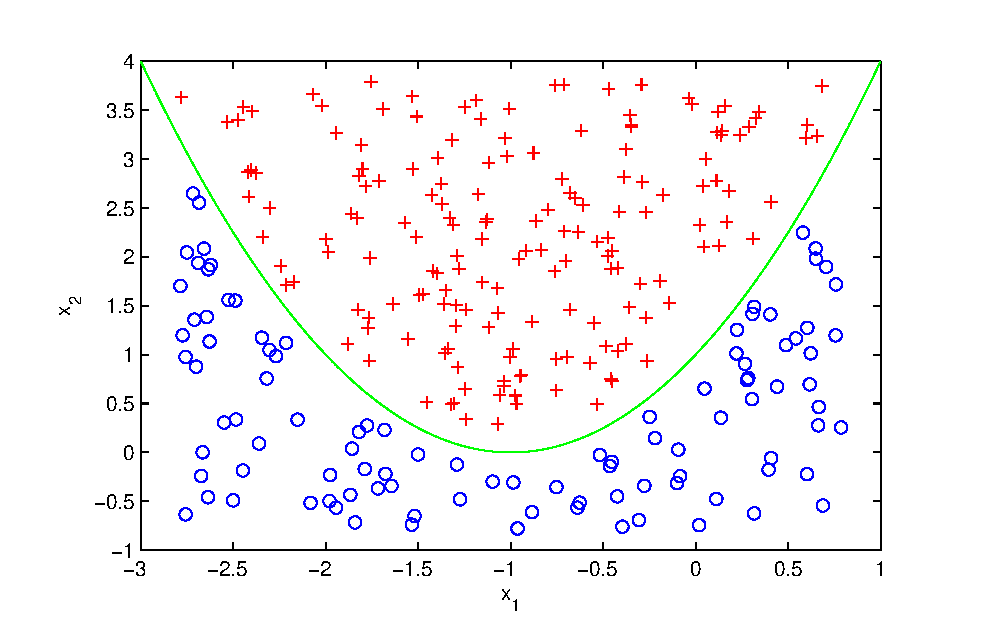
\includegraphics[width=0.50\textwidth]{images/fig21_featuresspace.eps}
\caption{
Configuration space vs. feature space. In this figure, the configuration space is $(x_1, x_2) \in \R^2$. The two classes are clearly separable by the green parabola, which is not linear. However, a linear binary classification model is able to separate the two classes as well using the (homogeneous) feature space $(1, x_1, x_1^2, x_2)$ and the weight vector $\w = (1, 2, 1, -1)$, both in $\R^4$.   
}
\label{fig:featuresspace}
\end{figure}


The goal of binary classification is to predict the class $\hat{t} \in \{ -1, 1 \}$ of a new observation $\x$. Linear binary classification achieves this by making a classification decision based on the value of a linear combination of the features. Specifically, the class prediction for $\x$ is based on the value of the following (so--called) predictor function \cite{bishop06}: 
\begin{equation} 
\label{eq:predictor}
f_{\w}(\x) = \sum_{j=1}^D w_j x_j + w_0 = \w^T \x + w_0,
\end{equation}
where $w_j$ is the weight corresponding to the $j-$th feature, $\w$ is the weight vector consisting of these individual weights, and $w_0$ is a bias (the negative of the bias is sometimes called a $threshold$). If $f_{\w}(\x) \geq 0$, the class prediction for $\x$ is $\hat{t} = 1$, otherwise $\hat{t} = -1$. Thus, the equation of the decision boundary that separates the two classes is $f_{\w}(\x) = \w^T \x + w_0 = 0,$
which is a hyperplane in this linear model (hence the decision boundary is also called \emph{decision hyperplane}). For convenience, the bias term is often included in the weight vector as $\begin{pmatrix}
w_0\\ \w \end{pmatrix}$, and the feature space is extended appropriately by a constant feature as $\begin{pmatrix} 1\\ \x \end{pmatrix}$. In this new notation, both $\w$ and $\x$ are in $\R^{D+1}$, and the predictor function is now $$f_{\w}(\x) = \w^T \x.$$ The equation of the decision hyperplane is now $$\w^T \x = 0,$$ which is a homogeneous system of equations. For this reason, this notation is called \emph{homogeneous}. For latter reference we call the former notation (with a separate bias $w_0$) \emph{non-homogeneous}. 

Note that the linear classification model may seem simple, but it can solve complicated problems as shown by Figure \ref{fig:featuresspace}, and is arguably the most commonly used classification model in practice. 

Clearly, to predict the class of a new observation, the weight vector $\w$ must have been already determined using a set of some ``historical'' observations with known class. In machine learning, this set is called the \emph{training dataset}, and contains some $N$ observations $\X = \{\boldsymbol{x_1, x_2, \dots, x_N}\}$ and their corresponding class $\t = \{t_1, t_2, \dots, t_N\}$. To measure the degree of belief in class prediction for an observation $\xi \in \X$, the so--called \emph{margin} is defined as follows:
\begin{equation} 
\label{eq:margin}
m_i(\w) = t_i f_{\w}(x_i),
\end{equation}
where $m_i(\w)$ is the margin corresponding to $\xi$. It can be seen that if $m_i(\w) < 0$ then the sign of the predictor function $f_{\w}(x_i)$ is opposite to the sign of then known class $t_i$ of point $\xi$, hence $\xi$ is misclassified. In this case, $m_i$ is a measure of the margin by which the class prediction for $\xi$ given by $f_{\w}(x_i)$ is wrong. Otherwise, if $m_i(\w) \geq 0$, then $\xi$ is correctly classified and $m_i$ represents the ``margin of safety'' by which the prediction is correct \cite{McAllester}.  

The task of classification is now boiled down to determine $\w$ based on the training dataset so as to minimize the sum of losses, where each loss quantifies the penalty for an incorrect classification in the training dataset. There are different types of losses used by different algorithms, such as 0--1 loss, log loss, squared loss, hinge loss, etc. Naturally, all these losses depend on the margin defined above, so the task is mathematically summarized as:
\begin{equation}
\label{eq:objective}
 \w^* = \arg\min_{\w} \; \sum_{i=1}^{N} L(m_i(\w)) + \lambda R(\w),
\end{equation}
where $L(m_i(\w))$ is some loss defined as a function of $m_i(\w)$, and the term $\lambda R(\w)$ is called the \emph{regularization term}, which prevents overfitting and extreme values of $\w$. In this term, $\lambda > 0$ is the \emph{regularization parameter}, which is tuned so as to maximize empirical performance of the resulting value of $\w^*$, and $R(\w)$ is the \emph{regularization function}, often defined as the $p-$norm of $\w$: 
$$R(\w) = \| \w \|_p = (\sum_{i=1}^D |w_i|^p)^{1/p}.$$
For instance, $p=1$ corresponds to the so--called $L_1$ regularizer: $$L_1(\w) = \sum_{i=1}^D |w_i|,$$ 
and $p=2$ corresponds to $L_2$ regularizer: $$L_2(\w) = \frac{1}{2} \w^T \w,$$ where the constant $\frac{1}{2}$ is added just for convenience, etc. 

We next review 0--1 loss and formulate the 0--1 loss optimization problem for linear binary classification. Other types of losses as well as their advantages and disadvantages shall be discussed in Section \ref{sec:bgr.surrogates}.   


%======================
\subsubsection{0--1 Loss and Problem Definition}
\label{ssec:01loss}

The 0--1 loss is defined for some margin $m$ as 
$$
L_{01}(m) = \left\{
     \begin{array}{ll}
       0 & : \text{if }m > 0\\
       1 & : \text{otherwise}
     \end{array}
   \right.
   \; = \; \mathbb{I} [m \leq 0],
$$
where the indicator function, $\mathbb{I} [.]$, is used to simplify the piecewise function. In the context of linear binary classification given in previous subsection, the margin is given by Equation \ref{eq:margin}, and the objective given by Equation \ref{eq:objective} now becomes
\begin{equation}
\label{eq:objective01}
 \w^* = \arg\min_{\w} \; \sum_{i=1}^{N} \mathbb{I} [t_i \w^T \xi \leq 0] + \lambda R(\w),
\end{equation}

It can be seen that in the context of 0--1 loss, the regularization term of the above objective function has no meaning as it can be always driven to zero by scaling down the weight vector $\w$ to $\epsilon \w$ with an arbitrarily small real positive constant $\epsilon$ without changing the 0--1 loss value, because the indicator function is invariant to such scaling. We can therefore omit this term, noting that in practice we can avoid overfitting by checking the components of $\w$ directly. The objective function now becomes
\begin{equation}
\label{eq:objective01}
 \w^* = \arg\min_{\w} \; \sum_{i=1}^{N} \mathbb{I} [t_i \w^T \xi \leq 0],
\end{equation}
where the sum of all losses $\sum_{i=1}^{N} \mathbb{I} [t_i \w^T \xi \leq 0]$ is called the 0--1 loss function. It can be seen, that the 0--1 loss function essentially counts the number of misclassifications. In this sense, 0--1 loss is the most natural loss function, because minimizing it is equivalent to minimizing the misclassification rate for the training data.

The subsequent chapters of this thesis study different approaches to optimize the 0--1 loss function. It is therefore convenient to give a unified problem definition for later reference as follows.

\begin{framed}
\label{definition}
{\bf The 0--1 Loss Optimization Problem Definition:}

\line(1,0){217}

Given a training dataset of $N$ observations $\X = \{\boldsymbol{x_1, x_2, \dots, x_N}\}$ and their corresponding targets $\t = \{t_1, t_2, \dots, t_N\}$, where  $\xi =  (1, x_{i1}, x_{i2}, \dots, x_{iD})^T \in \R^{D+1}$ and $t_i \in \{ -1, 1 \}$ for $i=1,2,\dots, N$. 

Find a weight vector $\w^*$, which minimizes the following 0--1 loss function:
\begin{equation}
\label{01loss}
L(\w) = \sum_{i=1}^N \mathbb{I} [t_i \w^T \xi \leq 0]
\end{equation}
where $\mathbb{I}$ is the indicator function, ${\w} = (w_0, w_1, \dots, w_D)^T \in \R^{D+1}$ is the (vector) variable of the 0--1 loss function $L(\w)$, and the task is to find (or approximate) 
$${\w}^* = \arg\min_{\w} L({\w})$$
\end{framed}

%=================================================
\subsection{Convex Optimization}
\label{sec:bgr.convexopt}

The objective function of the binary classification problem given by Equation \ref{eq:objective} is an optimization problem. Convex surrogates of 0--1 loss are often used in this objective function to gain computational efficiency. Thus, in this section we review gradient descent -- one of the first methods for convex optimization, keeping in mind that there are better methods like conjugate gradient, pseudo-Newton, etc., which are not in the scope of this thesis. A modified version of gradient descent called stochastic gradient descent is also reviewed. This version is suitable for situations where not all data are available at once. 

%======================
\subsubsection{Gradient Descent}

The convex optimization problem is defined as 
$$ \w^* = \arg \min_{\w} f(\w),$$
where $f(\w)$ is a convex function. 

The gradient descent method \cite{Cauchy} is based on the observation that if $f(\w)$ is defined and differentiable in a neighborhood of a point $\boldsymbol{a}$, then $f(\w)$ decreases fastest if one goes from $\boldsymbol{a}$ in the direction of the negative gradient of $f$ at $\boldsymbol{a}$, $-\nabla f(\boldsymbol{a})$. It follows that, if $\boldsymbol{b} = \boldsymbol{a} - \alpha \nabla f(\boldsymbol{a})$ for $\alpha \rightarrow 0$ a small enough number, then $f(\boldsymbol{a}) \geq f(\boldsymbol{b})$. With this observation in mind, the gradient descent method starts with a guess $\w^{(0)}$ and gradually updates it using 
$$\w^{(\tau + 1)} := \w^{(\tau)} - \alpha_{\tau} \nabla f(\w^{(\tau)}), $$
where $n \geq 0$, and the step size $\alpha_{\tau}$ is allowed to change in each step $\tau$. Then we have, 
$$f(\w^{(0)}) \geq f(\w^{(1)}) \geq f(\w^{(2)}) \geq \dots \;$$
Under the assumptions that $f(\w)$ is convex and $\nabla f(\w)$ Lipschitz, the sequence $(\w^{(\tau)})$ has been shown to converge to a local minimum, and because $f$ is convex, a local minimum is also global minimum. Thus, $(\w^{(\tau)})$ converges to the global solution $\w^*$.

%======================
\subsubsection{Stochastic Gradient Descent}
\label{ssec:sgd}

In machine learning, it often arises that the objective function is in the form
$$ \w^* = \arg \min_{\w} \sum_{i=1}^N f_i(\w),$$
where each function $f_i(.)$ is associated with the $i-$ observation of the training dataset. An example is the objective function for linear binary classification given by Equation \ref{eq:objective}. If the standard gradient descent is used to solve for $\w^*$, it is called \emph{batch learning}, and the update formula is 
$$\w^{(\tau +1)} := \w^{(\tau)} - \alpha \sum_{i=1}^N \nabla f_i(\w^{(\tau)}).$$

However, when the training dataset is big, the evaluation of the sum of gradients may become very expensive (due to limited availability of memory). In this case, stochastic gradient descent \cite{Davidon} is used to reduce the computational cost at every iteration, as it only samples a subset of summand functions' gradients. In this sense, it is also called \emph{online learning} or \emph{sequential learning}. In this case the update formula is 
$$\w^{(\tau +1)} := \w^{(\tau)} - \alpha \nabla f_i(\w^{(\tau)}).$$
We see that the individual gradient of an observation is used to approximate the sum of gradients. Often several passes over the training dataset are made until the algorithm converges. It has been shown by \cite{Bottou} and \cite{Kiwiel}, that when the learning rates decrease with an appropriate rate, and subject to relatively mild assumptions, stochastic gradient descent converges almost surely to a global minimum when the objective function is convex, and otherwise converges almost surely to a local minimum. 

%=================================================
\subsection{Surrogates of 0--1 Loss for Binary Classification}
\label{sec:bgr.surrogates}

In previous section we have reviewed the binary classification problem and 0--1 loss, minimizing which is equivalent to minimizing the error rate in the training dataset. However, direct optimization of 0--1 loss is NP--hard \cite{Feldman,nphard}, hence existing algorithms use convex surrogates of 0--1 loss. In this section, we first discuss the advantages and disadvantages of using a surrogate of 0--1 loss, and then review some of the most popular  surrogates and algorithms using them. Note that here we make heavy use of \cite{McAllester}, \cite{Webers}, \cite{bishop06}, and references therein.


%======================
\subsubsection{Advantages and Disadvantages of Surrogates}
\label{ssec:disadvantages}

Most state-of-the-art algorithms use some convex surrogate of 0--1 loss to solve the binary classification problem, because the convexity makes them computationally efficient \cite{Bartlett} and non-convexity often results in NP-hard problems. However, this choice comes at a cost as the disadvantages of convex objectives are well understood. Intuitively, loss should be bounded as we should not pay an infinite cost for misclassifying any one observation. It can be seen in Figure \ref{fig:losses}, that 0--1 loss is bounded, while other convex surrogates are not bounded with large negative margins. Because of this reason, \cite{outliers} showed that convex loss functions cannot be made robust in the presence of  noise. \cite{outliers2} further characterized this effect by analyzing various convex losses and found that risk minimization under 0-1 loss function has impressive noise tolerance properties and that under squared error loss is tolerant only to uniform noise; risk minimization under other loss functions is not noise tolerant.

%======================
\subsubsection{Squared Loss and Linear Regression}

The squared loss is defined as follows:

\[ \begin{split}
L_2(m_i(\w)) &= \frac{1}{2}[m_i(\w) - 1]^2 \\
& = \frac{1}{2}[t_i f_{\w}(\xi) - t_i^2]^2 \\
& = \frac{1}{2}t_i^2 [f_{\w}(\xi) - t_i]^2 \\
& = \frac{1}{2}[\w^T\xi - t_i]^2,
\end{split} \] 
where we used the fact that $t_i^2 = 1$, and the constant $\frac{1}{2}$ is used for later convenience. We see that minimizing (the sum of) squared loss is equivalent to minimizing the (total squared) difference between the value given by the predictor function $\w^T\xi$ and the training target $t_i$. By applying this loss to the objective function of binary classification given by Equation \ref{eq:objective01} we have the following:
\begin{equation}
\label{eq:squareobj}
\w^* = \arg\min_{\w} \; \sum_{i=1}^{N}  \frac{1}{2}[\w^T\xi - t_i]^2 + \lambda R(\w).
\end{equation}
Squared loss is often used with $L_2$ or $L_1$ regularizers. It is called \emph{ridge regression} if used with $L_2$ regularizer, or \emph{lasso} if used with $L_1$. We further consider ridge regression (keeping in mind that lasso is similar), in this case the objective function becomes 
\[ \begin{split}
\w^* & = \arg\min_{\w} \;  \frac{1}{2} \sum_{i=1}^{N} [\w^T\xi - t_i]^2 + \frac{\lambda}{2} \w^T\w \\
& = \arg\min_{\w} \; \{  \frac{1}{2}(\t - \X\w)^T(\t - \X\w) + \frac{\lambda}{2} \w^T\w \},
\end{split} \]
where 
$\t = \begin{pmatrix} t_1\\ t_2 \\ \vdots \\ t_N \end{pmatrix}$, and 
$\X = \begin{pmatrix} \boldsymbol{x_1}\\ \boldsymbol{x_2}\\ \vdots \\ \boldsymbol{x_N}\end{pmatrix}$. 
Let $g(\w)$ denote the function to be optimized: 
$$ g(\w) = \frac{1}{2}(\t - \X\w)^T(\t - \X\w) + \frac{\lambda}{2} \w^T\w.$$
This is a convex function and there are two ways to optimize it: analytical and sequential, both are addressed as follows.

For the \emph{analytical solution}, we calculate the gradient of $g(\w)$ and set it to zero: 
\[ \begin{split}
& \nabla g(\w) = \X^T(\X\w - \t) + \lambda\w = \boldsymbol{0}  \\
\Leftrightarrow \quad & (\X^T \X + \lambda \boldsymbol{I}) \w = \X^T \t \\
\Leftrightarrow \quad & \w^* = (\X^T\X + \lambda \boldsymbol{I})^{-1}\X^T \t, 
\end{split} \]
where $\boldsymbol{I}$ denotes the identity matrix. It is easy to check that the Hessian matrix $$H(g) = \X^T\X + \lambda \boldsymbol{I}$$ is positive semi definite, so $\w^*$ is a local minimum. As $g(\w)$ is convex, $\w^*$ is also the global minimum. Thus, $\w^* = (\X^T\X + \lambda \boldsymbol{I})^{-1}\X^T \t$ is the \emph{closed form solution} to the objective function given by Equation \ref{eq:squareobj}.

For big datasets, however, the calculation of the given closed form solution of $\w^*$ may be very expensive. In this case, the \emph{online learning} approach is used by applying the stochastic gradient descent method discussed in Subsection \ref{ssec:sgd}. The concrete \emph{linear regression} procedure is given as follows. 
\begin{description}
\setlength{\itemsep}{0cm}
\setlength{\parskip}{0cm}
\item[Step 1:] \hfill \\initialize $\w$ to some initial value
\item[Step 2:] \hfill \\update $\w$ in each iteration by: 
$$\w := \w - \alpha (\nabla L(m_i(\w)) + \lambda \w)$$
\end{description}
where $\nabla L(m_i(\w))$ is the gradient of an individual loss, in this case the squared loss of the $i-$th point:
$$\nabla L(m_i(\w)) = (\w^T \xi - t_i)\xi,$$
and the step size $\alpha$ (also called \emph{learning rate}) must be chosen carefully, as a too large learning rate prevents algorithm from converging and a too small learning rate updates $\w$ too slowly. Often several passes over the training set are made until the algorithm converges. Typical implementations may also randomly shuffle training examples at each pass and use an adaptive learning rate.

%======================
\subsubsection{Log Loss and Logistic Regression}

We have discussed in Subsection \ref{ssec:binclass}, that if $m_i < 0$ then $|m_i|$ is a measure of the margin by which the class prediction for $\xi$ given by $f_{\w}(x_i)$ is wrong, otherwise the prediction is correct. In this sense, the log loss is defined as 
\[ \begin{split}
L_{log}(m_i(\w)) &= \ln (1 + e^{-m_i(\w)}) \\
 &= \ln (1 + e^{-t_i\w^T\xi}) 
\end{split} \] 
It can be easily verified, that this loss is convex, and for $m_i >> 1$ we have $L_{log}(m_i) \approx 0$, on the other hand, for $m_i << -1$ we have $L_{log} \approx -m_i = |m_i|$. In other words, log loss is a convex model of the scheme, where misclassification is penalized by the absolute value of the margin, and correct classification has zero penalty. We note that both log loss and quadratic loss can be viewed as an attempt to estimate $P(t|\x)$ and can be derived under assumption that $P(\x|t)$ has (multivariate) Gaussian distribution. However, for the purpose here we will not go into this detail. By applying log loss to the objective function of binary classification given by Equation \ref{eq:objective01} we have the following:
\begin{equation}
\label{eq:logobj}
\w^* = \arg\min_{\w} \; \sum_{i=1}^{N} \ln(1 + e^{-t_i\w^T\xi})  + \lambda R(\w).
\end{equation}

\emph{Logistic regression} is the combination of log loss with $L_2$ regularizer, where the objective function becomes 
\[ \begin{split}
\w^* & = \arg\min_{\w} \; \sum_{i=1}^{N} \ln(1 + e^{-t_i\w^T\xi}) + \frac{\lambda}{2} \w^T\w \\
\end{split} \]

In contrast to the previous case, this time there is no closed form solution for $\w^*$. So we have to revert to an iterative procedure, e.g., batch learning or online learning discussed in Subsection \ref{ssec:sgd}. A concrete regression procedure has been given in the previous subsection. Here for completeness, we will derive the update form. Let $g(\w)$ denote the function to be optimized:
$$ g(\w) = \sum_{i=1}^{N} \ln(1 + e^{-t_i\w^T\xi}) + \frac{\lambda}{2} \w^T\w.$$
Then its gradient is 
\[ \begin{split}
 \nabla g(\w) &= \sum_{i=1}^{N} \frac{1}{1+e^{-t_i \w^T \xi}}e^{-t_i \w^T \xi} (-t_i \xi) + \lambda \w \\
 &= - \sum_{i=1}^{N} \frac{1}{1 + e^{t_i \w^T \xi}} t_i \xi + \lambda \w \\
 &= - \sum_{i=1}^{N} \sigma(-m_i(\w)) \, t_i \xi + \lambda \w,
\end{split} \]
where $\sigma(a) = \frac{1}{1 + exp(-a)}$ is called the logistic sigmoid function. With the gradient available, it is now easy to derive the update form. For batch learning it is
$$\w := \w + \alpha \sum_{i=1}^{N} \sigma(-m_i(\w)) \, t_i \xi - \alpha \lambda \w.$$
And for online learning it is
$$\w := \w + \alpha \, \sigma(-m_i(\w)) \, t_i \xi - \alpha \lambda \w.$$
Note that for a same training dataset, the regularization constant $\lambda$ for online learning would be much smaller than that for batch learning. 


%======================
\subsubsection{Hinge Loss and Support Vector Machine}

The hinge loss is defined as
\[ \begin{split}
L_{hinge}(m_i(\w)) &= \max(0, 1 - m_i(\w)) \\
&= \max(0, 1 - t_i \w^T \xi),
\end{split} \] 
and it can be viewed as a piecewise linear approximation of log loss, because it has the same properties as given for log loss for cases when $m_i >> 1$ and $m_i << -1$. Although being convex, this loss is difficult to optimize directly using the traditional procedure. To be more specific, applying this loss with $L_2$ regularizer to Equation \ref{eq:objective} yields 
\begin{equation}
\label{eq:svmobj}
\w^* = \arg\min_{\w} \; \sum_{i=1}^{N} \max(0,1 - t_i\w^T\xi)  + \frac{\lambda}{2} \w^T\w,
\end{equation}
which is non--differentiable, so typical optimization methods cannot be directly applied. However, the support vector machines (SVM) method proposed by \cite{Vapnik} minimizes this loss by using the maximum-margin classification approach, which we briefly review the key points of this method as follows.

First, suppose that the two classes of the discussed linear binary classification problem are linearly separable by some weight vector $\w$. Then, SVM chooses the decision boundary which maximizes the smallest distance to samples in both classes, which is mathematically defined as
$$ \w^* = \arg \max_{\w} \{ \frac{1}{\|\w\|} \min_i [t_i\w^T \xi] \}. $$
We have discussed in Subsection \ref{ssec:01loss}, that scaling $\w$ to $\epsilon \w$ does not change the decision hyperplane. Thus we can scale $\w$ in such a way that for the closest point $t_i\w^T \xi = 1$. Then the objective function becomes 
\[ \begin{split}
& \w^* = \arg \max_{\w} \{ \frac{1}{\|\w\|} \} \quad s.t. \quad \;t_i\w^T \xi \geq 1 \quad \forall i = 1, 2, \dots, N \\
\Leftrightarrow \quad &  \w^* = \arg \min_{\w} \{ \frac{1}{2}\|\w\|^2 \} \quad s.t. \quad \;t_i\w^T \xi \geq 1 \quad \forall i = 1, 2, \dots, N.
\end{split} \] 
This is a quadratic programming problem: minimize a quadratic function subject to linear constraints, and can be efficiently solved using the method of Lagrange multipliers with the Karush�Kuhn�Tucker (KKT) conditions \cite{Kuhn}. 

Now, for the case when the two classes are not linearly separable, hinge loss is used to penalize data points that are on the `wrong side' of the decision boundary as follows:
$$L_{hinge}(m_i) 
\left\{
     \begin{array}{ll}
       = 0 & : \xi \text{ is correctly classified and on or beyond the margin}\\
       < 1 & : \xi \text{ is in the correct margin}\\
       = 1 & : \xi \text{ is on the decision boundary}\\
       > 1 & : \xi \text{ is misclassified, penalty } \approx |m_i|
     \end{array}
   \right..
$$
The constraints are now changed to 
$$ t_i\w^T \xi \geq 1 - L_{hinge}(m_i) \quad \forall i = 1, 2, \dots, N,$$
and the objective is to minimize 
$$ C \sum_{i=1}^N L_{hinge}(m_i) + \frac{1}{2} \w^T\w,$$  
where the constant $C$ controls the trade-off between the loss and the margin. To sum up, the full objective function is:
\[ \begin{split}
\w^* = \arg\min_{\w} \{ C \sum_{i=1}^N  \max(0, 1 - t_i \w^T \xi) + \frac{1}{2} \w^T\w \} \\
s.t. \quad t_i\w^T \xi \geq 1 - \max(0, 1 - t_i \w^T \xi) \quad \forall i = 1, 2, \dots, N.
\end{split} \] 
We see that this is, again, a quadratic programming problem, which can be solved efficiently as discussed before. Furthermore, this function is similar to the objective function given by Equation \ref{eq:svmobj}, with the only difference in the constants $\lambda$ and $C$, both of them, however, can be treated as a regularization constant.


%=================================================
\subsection{Other Methods for Binary Classification}
\label{sec:bgr.others}

In the previous section, we have reviewed some of the most popular methods for binary classification. In this section, we will briefly review some other methods that have not been mentioned. The first subsection is devoted to Bayes point machine. The subsequent subsection then summarizes several other methods.  

%======================
\subsubsection{Bayes Point Machine}

Bayes point machine (BPM) was proposed by \cite{Herbrich}. This is a Bayesian approach to linear classification and is briefly summarized as follows. From our discussion in Subsection \ref{ssec:binclass} we see that, in linear classification, a point $\x$ is classified by $t = \sign(\w^T \x)$ for some weight vector $\w$. Given the training dataset $\D = \{\X, \t \}$, the likelihood for $\w$ is given by
$$p(\D | \w) = \prod_{i=1}^N p(t_i | \xi, \w) = \prod_{i=1}^N \phi(\frac{t_i\w^T\xi}{\epsilon}),$$
where 
$$\phi(z) = \int_{-\infty}^z N(z; 0, 1) dz,$$
and $\epsilon$ controls the allowed `slack'. By using $\phi$ instead of a step function, this likelihood tolerates small errors. Under the Bayesian approach, we also have a prior distribution of $\w$, which is taken to be the zero-mean unit-variance normal distribution: $N(\boldsymbol{0, I})$. Given this model, the optimal way to classify a new data point $\x$ is to vote all classifiers according to their posterior probability: $\mathbb{E}[\sign(\w^T \x) | \D]$. This is, however, expensive to compute. As an approximation to this, BPM uses the output of the average classifier: $\sign(\mathbb{E}[\w] ^T \x)$. This can be estimated by the billiard ball algorithm proposed in the original BPM paper, which is based on the Monte Carlo method. Another (better) way to estimate this is by using expectation propagation as proposed by \cite{bpm}. This thesis uses the Matlab implementation of expectation propagation algorithm for BPM of the latter author in all comparisons where BPM is present. 

%======================
\subsubsection{Other Methods}

Apart from mentioned algorithms, there are quite a few other algorithms that can solve the binary classification problem. Some of the most notable are, for example, the following. Neural networks \cite{bishop2} consist of one or more interconnected layers of neurons, each neuron having its own weight vector. It can be viewed as an adaptive system that changes its structure during learning phase. In contrast to the introduced linear binary classification model, neural networks is generally not linear, except for perceptrons \cite{perceptron}, which can be considered as the simplest kind of neural network. Perceptron, however, may not converge if the two classes are not linearly separable. $k-$ Nearest Neighbor \cite{kNN} is one of the simplest classification algorithms. It assigns a new data point to the class most common amongst its $k$ nearest training data points (neighbors). Adaboost \cite{adaboost}, short for Adaptive Boosting, is an algorithm that coordinate several weak classifiers to improve the classification quality, where subsequent classifiers are tweaked in favor of those instances misclassified by previous classifiers. Adaboost uses exponential loss, which is $L_{exp} = \exp(-m_i(\w)) = \exp(-t_i\w^T\xi)$, hence can be sensitive to noisy data and outliers. Decision trees are also used for classification as shown by \cite{tree1}, and by \cite{tree2}. 

There are also many works that are more or less related to the work of this thesis. We can categorize them into those developing classifiers that are robust to outliers and those optimizing 0--1 loss directly. The number of works in the first category is quite abundant, including t-logistic regression \cite{Ding}, robust truncated hinge loss \cite{robusthinge}, SavageBoost \cite{lossdesign}, and more. There are, however, almost no works in the second category. At the time of finishing this thesis, we can only find the work by \cite{ling}, which proposes an algorithm optimizing 0--1 loss for perceptrons by random coordinate descent. 


%=================================================
\subsection{Summary}
\label{sec:bgr.summary}

In this chapter, we have reviewed the linear binary classification problem and several popular methods for it. However, these methods depend on convex surrogates of 0--1 loss, hence suffer from the presence of noise and outliers in the training set as discussed in Subsection \ref{ssec:disadvantages}. One strategy to avoid this problem is to optimize 0-1 loss directly, and this is the topic of study in the remaining chapters of the thesis. 

%%% Local Variables: 
%%% mode: latex
%%% TeX-master: "thesis"
%%% End: 
